% The orthogonality centre sits on a site or on a bond, and the notation has to
% say both, because the two are one SVD apart and a method moves between them
% every sweep.
%
% Above: the centre on a site. C carries a physical index like every other
% tensor on the chain, and is the only one that is not isometric.
%
% Below: the centre on a bond. Take C = U Lambda V^dagger, absorb U into the
% site on its left and V^dagger into the site on its right, and both of those
% become isometric -- so the chain is A A A to the left and B B to the right,
% five sites still, and what is left over is Lambda, which lives between two
% sites and carries no physical index. Those are the Schmidt values across that
% cut, which is why this form is the one to read an entanglement spectrum off.
%
% Same diamond for both, because it is the same object in the same role; what
% differs is the slot it sits in, and a bond slot is narrower than a site one.
% Lambda takes a slot of the row like anything else, so the lower line is one
% slot longer than the upper -- written as that, relative to the upper line's
% own ends, rather than as a second set of coordinates.
%
% Finite, so the chain simply stops: the outer indices are open, with nothing at
% the far end, and drawn inward so their arrowheads run toward the centre.
\documentclass[border=4pt]{standalone}
\usepackage{amsmath,amssymb}
\usepackage{tikz-tensors}
\begin{document}
\begin{tikzpicture}[x=1.35cm]
  % ---- the centre on a site ----------------------------------------------
  \tnchain{S}{(0,0)}{(5.2,0)}{canl/$A$/l, canl/$A$/l, centre/$C$/c,
                            canr/$B$/r, canr/$B$/r}
  \tnbond[gauge]{(S1) -- (S2)}  \tnbond[gauge]{(S2) -- (S3)}
  \tnbond[gauge]{(S5) -- (S4)}  \tnbond[gauge]{(S4) -- (S3)}
  \tnbond[gauge]{([xshift=-5mm]S1.west) -- (S1)}
  \tnbond[gauge]{([xshift=5mm]S5.east) -- (S5)}
  \tnlegs{10mm}{S1-leg,S2-leg,S3-leg,S4-leg,S5-leg}
  \foreach \i in {1,...,5} \tnput[below]{S\i-leg-tip}{$n_{\i}$};

  % ---- the centre on the bond between sites 3 and 4 ----------------------
  % One slot longer, and placed from the line above rather than from scratch.
  \tnchain{T}{($(S1)+(0,-2.6)$)}{($(S5)+(1.3,-2.6)$)}%
             {canl/$A$/l, canl/$A$/l, canl/$A$/l,
              centrebond/$\Lambda$/c, canr/$B$/r, canr/$B$/r}
  \tnbond[gauge]{(T1) -- (T2)}  \tnbond[gauge]{(T2) -- (T3)}
  \tnbond[gauge]{(T3) -- (T4)}  \tnbond[gauge]{(T5) -- (T4)}
  \tnbond[gauge]{(T6) -- (T5)}
  \tnbond[gauge]{([xshift=-5mm]T1.west) -- (T1)}
  \tnbond[gauge]{([xshift=5mm]T6.east) -- (T6)}
  \tnlegs{10mm}{T1-leg,T2-leg,T3-leg,T5-leg,T6-leg}
  \foreach \s/\l in {1/1, 2/2, 3/3, 5/4, 6/5}
    \tnput[below]{T\s-leg-tip}{$n_{\l}$};
\end{tikzpicture}
\end{document}
